\chapter{Sinterizzazione}\label{chp:Sinterizzazione}
Permette di realizzare oggetti a partire da polveri di un
materiale.

\begin{quote}
\emph{Perché sfruttare la sinterizzazione?}
\end{quote}

I motivi sono molteplici e possono essere:
\begin{itemize}
\item controllo accurato della struttura richiesta;
\item controllo della composizione chimica;
\item formabilità;
\item Quando non si vogliono macrosegregazioni;
\item realizzare dei componenti in materiali con temperatura di 
fusione particolarmente alta.
\end{itemize}

A differenza di altre lavorazioni è necessario parametrizzare la 
forma delle polveri, in quanto da quei parametri si possono ottenere 
le caratteristiche meccaniche del lavorato finale.
Inoltre la forma della polvere può essere determinante sulla
lavorazione.

Per i prodotti lavorati in sinterizzazione si parla di \eng{Net-
Shape}: ovvero, la lavorazione porta dei semilavorati già molto 
vicini alla forma finale di vendita del prodotto.
Ciò permette di usare tutto il materiale, senza avere sprechi dovuti
a delle lavorazioni che per ottenere la forma finale, devono 
eliminare parte di esso.

Data la lavorazione è possibile controllare la porosità del prodotto
come si vedrà successivamente.
In generale non si ottengono particolari caratteristiche meccaniche
anche se alle volte si possono ottenere delle caratteristiche 
migliori di altre lavorazioni già viste.

Bisogna prestare attenzione al discorso della porosità: troppa
porosità residua può essere punto di fragilità del materiale portando
alla formazione di cricche.
In più non sono facili da lavorare in post-produzione. Quindi il 
processo di produzione deve essere \eng{near net-shape} il più
possibile.

\section{La lavorazione}
Alla figura \ref{fig:ProcSint} sono riportati i principali
possibili processi per le lavorazioni di sinterizzazione.

\begin{figure}
\centering
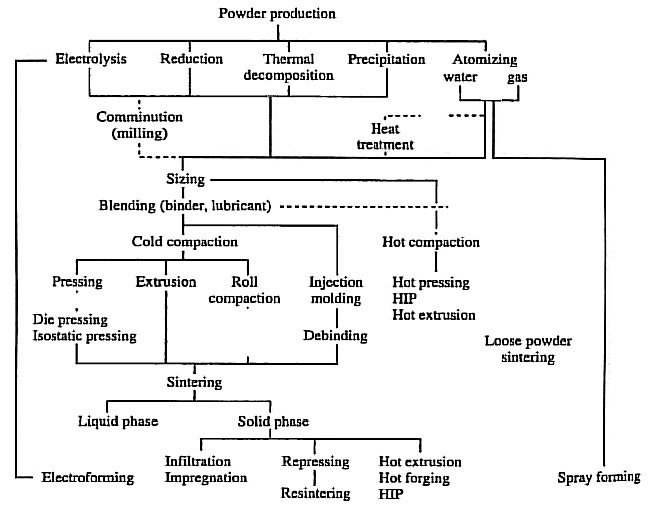
\includegraphics[width = \textwidth]{ProcSint}
\caption{Processi di produzione in sinterizzazione}
\label{fig:ProcSint}
\end{figure}

In generale il processo di sinterizzazione deve passare attraverso 
tre principali processi:

\begin{center}
\smartdiagramset{%
sequence item uniform color = UniFeLight!50,
sequence item width = 0.3\textwidth,
back arrow disabled=true}
\smartdiagram[sequence diagram]{Produzione Polveri, Compattazione, Sinterizzazione}
\end{center}

Sarà anche la la sequenza delle trattazioni successive.

\subsection{Produzione delle polveri}
